\chapter{Anexo I: Matriz de Consistencia}


\begin{table}[h!]
	\centering
	\small
	\begin{tabular}{ |m{5cm}|m{5cm}|m{5cm}|  }
		\hline
		\rowcolor{bluejean}
		\Centering \color{white}{PROBLEMAS}& \Centering \color{white}{OBJETIVOS}& \Centering \color{white}{HIPÓTESIS}\\
		\hline
		\rowcolor{turq}
		\Centering Problema General& \Centering Objetivo General & \Centering Hipótesis General \\
		\hline
		{\ProblemaGeneral} & { \ObjetivoGeneral} & {\HipotesisGeneral} \\
		\hline
		\rowcolor{turq}
		\Centering Problemas Específicos& \Centering Objetivos Específicos & \Centering Hipótesis Específicas \\
		\hline
		{\Pbone} & {\Objone} & {\Hone} \\
		\hline
		{\Pbtwo} & {\Objtwo} & {\Htwo} \\
		\hline
		{\Pbthree} & {\Objthree} & {\Hthree} \\
		\hline
		{\Pbfour} & {\Objfour} & {\Hfour} \\
		\hline

	\end{tabular}
	\caption{Matriz de consistencia. Fuente: Elaboración propia}
	\label{1:table}
\end{table}

\begin{table}[htbp]
    \centering
    \begin{tabular}{|p{4.5cm}|p{4.5cm}|p{6cm}| }
        \toprule
        \Centering \textbf{Hipótesis Específica} & \Centering \textbf{Indicadores} & \Centering \textbf{Fórmulas} \\
        \midrule
        {\Hone} & 
        \begin{tabular}[t]{@{}p{4.3cm}@{}}
            $*$Porcentaje de integración de APIs \\
            $*$Calidad de datos\\
	     $*$Tiempo de respuesta de la API\\
	     $*$Porcentaje de consultas resueltas
        \end{tabular} & 
        \begin{tabular}[t]{@{}p{5.8cm}@{}}
		$\frac{\text{Número de APIs integradas}}{\text{Total de APIs disponibles}} \times 100$\\\\
            $\frac{\text{\tiny Cantidad de datos precisos y actualizados}}{\text{\tiny Total de datos utilizados}} \times 100$\\\\
            $\frac{\text{Tiempo total de respuesta de la API}}{\text{Número total de consultas}}$\\\\
		$\frac{\text{Consultas resueltas}}{\text{Total de consultas realizadas}} \times 100$
        \end{tabular} \\
        \midrule
         {\Htwo}  & 
        \begin{tabular}[t]{@{}p{4.3cm}@{}}
            $*$Precisión del modelo de lenguaje natural \\
            $*$Eficiencia del chatbot\\\\
		$*$Tasa de reconocimiento de entidades médicas\\
		$*$Cobertura de conocimiento médico
        \end{tabular} & 
        \begin{tabular}[t]{@{}p{5.8cm}@{}}
            $\frac{\text{Número de respuestas correctas}}{\text{Total de respuestas generadas}} \times 100$\\\\
            $\frac{\text{Número de consultas manejadas}}{\text{Tiempo total de prueba}}$\\\\
            $\frac{\text{\tiny Número de entidades médicas correctamente identificadas}}{\text{\tiny Total de entidades médicas identificadas}} \times {\tiny 100}$\\
		$\frac{\text{\tiny Número de temas médicos cubiertos correctamente}}{\text{\tiny Total de temas médicos probados}} \times 100$
        \end{tabular} \\
        \midrule
        {\Hthree} & 
        \begin{tabular}[t]{@{}p{4.3cm}@{}}
            $*$Exactitud del conjunto de datos de entrenamiento \\\break
            $*$Tasa de generalización del modelo\\
		$*$Precisión de la validación cruzada\\
		$*$Estabilidad del modelo
        \end{tabular} & 
        \begin{tabular}[t]{@{}p{5.8cm}@{}}
            $\frac{\text{\tiny Número de pares de consulta-respuesta correctos}}{\text{\tiny Total de pares de consulta-respuesta}} \times 100$\\\\\\\break
            $\frac{\text{\tiny Número de consultas generales respondidas correctamente}}{\text{\tiny Total de consultas generales}} \times {\tiny 100}$\\
            $\frac{\text{\tiny Número de consultas validadas correctamente}}{\text{\tiny Total de consultas validadas}} \times 100$\\\\
		$\frac{\text{\tiny Desviación estándar del rendimiento del modelo}}{\text{\tiny Media del rendimiento del modelo}} \times 100$
        \end{tabular} \\
        \midrule
        {\Hfour} & 
        \begin{tabular}[t]{@{}p{4.3cm}@{}}
            $*$Reducción en tiempos de espera \\\\
            $*$Aumento en la accesibilidad de servicios médicos\\
	     $*$Mejora en la precisión del diagnóstico\\\\
	     $*$Satisfacción del usuario
        \end{tabular} & 
        \begin{tabular}[t]{@{}p{5.8cm}@{}}
		\tiny Antes= Tiempo promedio de espera antes de la implementación \break
		\tiny Despues= Tiempo promedio de espera después de la implementación\\
            $\frac{\text{\tiny Antes} - \text{\tiny Despues}}{\text{\tiny Antes}} \times 100$ \\\\
		$\frac{\text{\tiny Número de consultas médicas atendidas por el chatbot}}{\text{\tiny Total de consultas médicas realizadas}} \times 100$\\\\
		\tiny dChat=Precisión del diagnóstico del chatbot. \break
		\tiny dHumano=Precisión del diagnóstico humano\\
            $\frac{\text{\tiny dChat} - \text{\tiny dHumano}}{\text{\tiny dHumano}} \times 100$\\\\
		$\frac{\text{Número de usuarios satisfechos}}{\text{Total de usuarios encuestados}} \times 100$
        \end{tabular} \\
        \bottomrule
    \end{tabular}
 \caption{Tabla de Hipótesis Específicas, Indicadores y Fórmulas}
    \label{tab:hipotesis}
\end{table}


\chapter{Anexo II: Arbol del Problema}
%\section{Conclusiones}

\begin{figure}[h]
	\begin{center}
		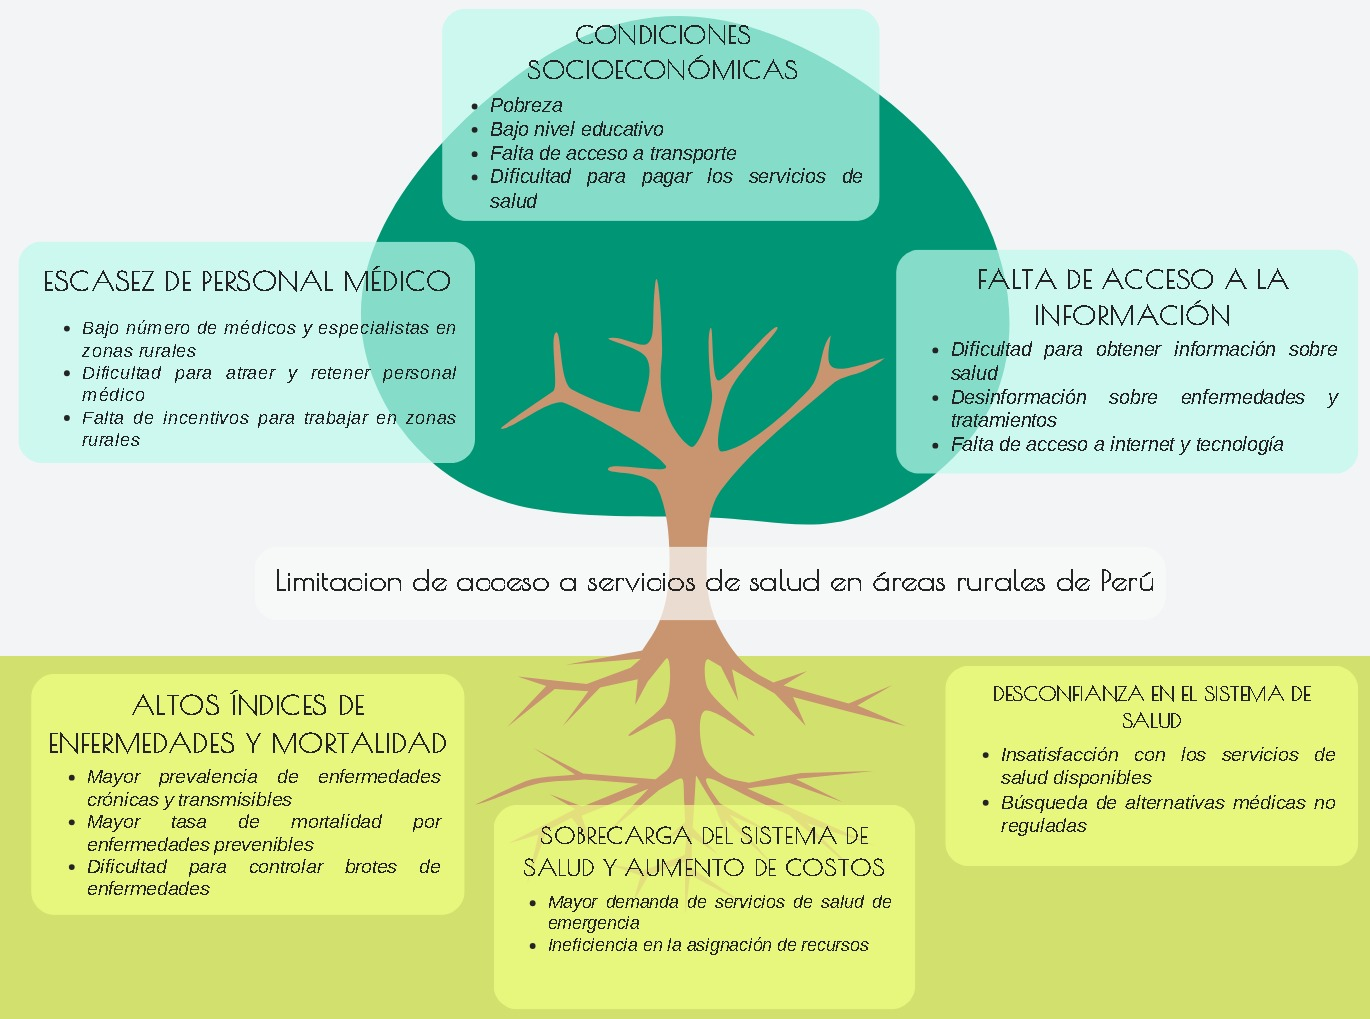
\includegraphics[width=0.8\textwidth]{images_repo/Arbol del problema.jpeg}
		\caption{Árbol del problema. Fuente: Elaboración propia}
		\label{1:fig}
	\end{center}
\end{figure}

\chapter{Anexo III: Arbol de Objetivos}
%\section{Conclusiones}

%\begin{figure}[h]
%	\begin{center}
%		\includegraphics[width=0.6\textwidth]{images_repo/ArbolObjetivos.jpeg}
%		\caption{Árbol de objetivos. Fuente: Elaboración propia}
%		\label{1:fig}
%	\end{center}
%\end{figure}

\chapter{Anexo IV: Resumen de Papers investigados}
%\section{Conclusiones}

\begin{table}[h]
	\newcommand{\multirot}[1]{\multirow{2}{*}[-8ex]{\rotcell{\rlap{#1}}}}
	%\scriptsize
	\footnotesize
	\centering
	\begin{tabular}{|m{0.5cm}|m{0.3cm}|m{4cm}|m{2cm}|m{0.6cm}|m{1.7cm}|m{3cm}|} 
		\hline
		\rowcolor[rgb]{0,0.251,0.502} \multicolumn{1}{|c|}{\textcolor{white}{Tipo}} & \multicolumn{1}{c|}{\textcolor{white}{N°}} & \multicolumn{1}{c|}{\textcolor{white}{Título}}                                                                             & \multicolumn{1}{c|}{\textcolor{white}{Autor}}        & \multicolumn{1}{c|}{\textcolor{white}{Año}} & \multicolumn{1}{c|}{\textcolor{white}{País}} & \multicolumn{1}{c|}{\textcolor{white}{Fuente}}                                                        \\ 
		\hline
		\multirot{Problema}                                        & 1                                             & Copper price estimation using bat algorithm~                                                                               & Dehghani  Bogdanovic                                 & 2018                                        & United Kingdom                               & Resources Policy                                                                                      \\ 
		\cline{2-7}
		& 2                                             & Alternative techniques for forecasting mineral commodity prices                                                            & Cortez, Saydam, Coulton,  Sammut                     & 2018                                        & Netherlands                                  & International Journal of Mining Science and Technology                                                \\ 
		\hline
		\multirow{3}{*}[-14ex]{\rotcell{\rlap{Propuesta}}}
		& 3                                             & Prediction of the crude oil price thanks to natural language
		processing applied to newspapers~                           & Trastour, Genin,  Morlot                             & 2016                                        & USA                                          & Standfort University ML repository                                                                    \\ 
		\cline{2-7}
		& 4                                             & Stock Price Prediction Using Deep Learning~                                                                                & Tipirisetty                                          & 2018                                        & USA                                          & Master's Theses San Jose State University                                                             \\ 
		\cline{2-7}
		& 5                                             & Deep Learning for Stock Prediction Using Numerical and Textual
		Information                                               & Akita, R., Yoshihara, A., Matsubara, T.,  Uehara, K. & 2016                                        & USA                                          & 2016 IEEE/ACIS 15th International Conference on Computer and
		Information Science (ICIS)             \\ 
		\hline
		\multirow{4}{*}[-28ex]{\rotcell{\rlap{Técnica}}}                                          & 6                                             & Stock Prices Prediction using the Title of Newspaper Articles
		with Korean Natural Language Processing~                   & Yun, Sim,  Seok                                      & 2019                                        & Japan                                        & 2019 International Conference on Artificial Intelligence in
		Information and Communication (ICAIIC)  \\ 
		\cline{2-7}
		& 7                                             & A Method of Optimizing LDA Result Purity Based on Semantic
		Similarity                                                    & Jingrui, Z., Qinglin, W., Yu, L.,  Yuan, L.          & 2017                                        & China                                        & 2017 32nd Youth Academic Annual Conference of Chinese
		Association of Automation (YAC)~              \\ 
		\cline{2-7}
		& 8                                             & Qualitative Stock Market Predicting with Common Knowledge Based
		Nature Language Processing: A Unified View and Procedure & Rao, D., Deng, F., Jiang, Z.,  Zhao, G.~             & 2015                                        & USA                                          & 2015 7th International Conference on Intelligent Human-Machine
		Systems and Cybernetics              \\ 
		\cline{2-7}
		& 9                                             & Fuzzy Bag-of-Words Model for Document Representation                                                                       & Zhao, R.,  Mao, K.                                   & 2018                                        & USA                                          & IEEE Transactions on Fuzzy Systems (~Volume:
		26~,~Issue: 2~, April 2018~)                           \\
		\hline
	\end{tabular}
	\caption{Cuadro Resumen de Papers investigados. Fuente: Elaboración propia}
\label{A:table}
\end{table}



